\appendix{Simulation Appendix}
\section{Common Pool:}
\begin{figure}[h]
    \centering
    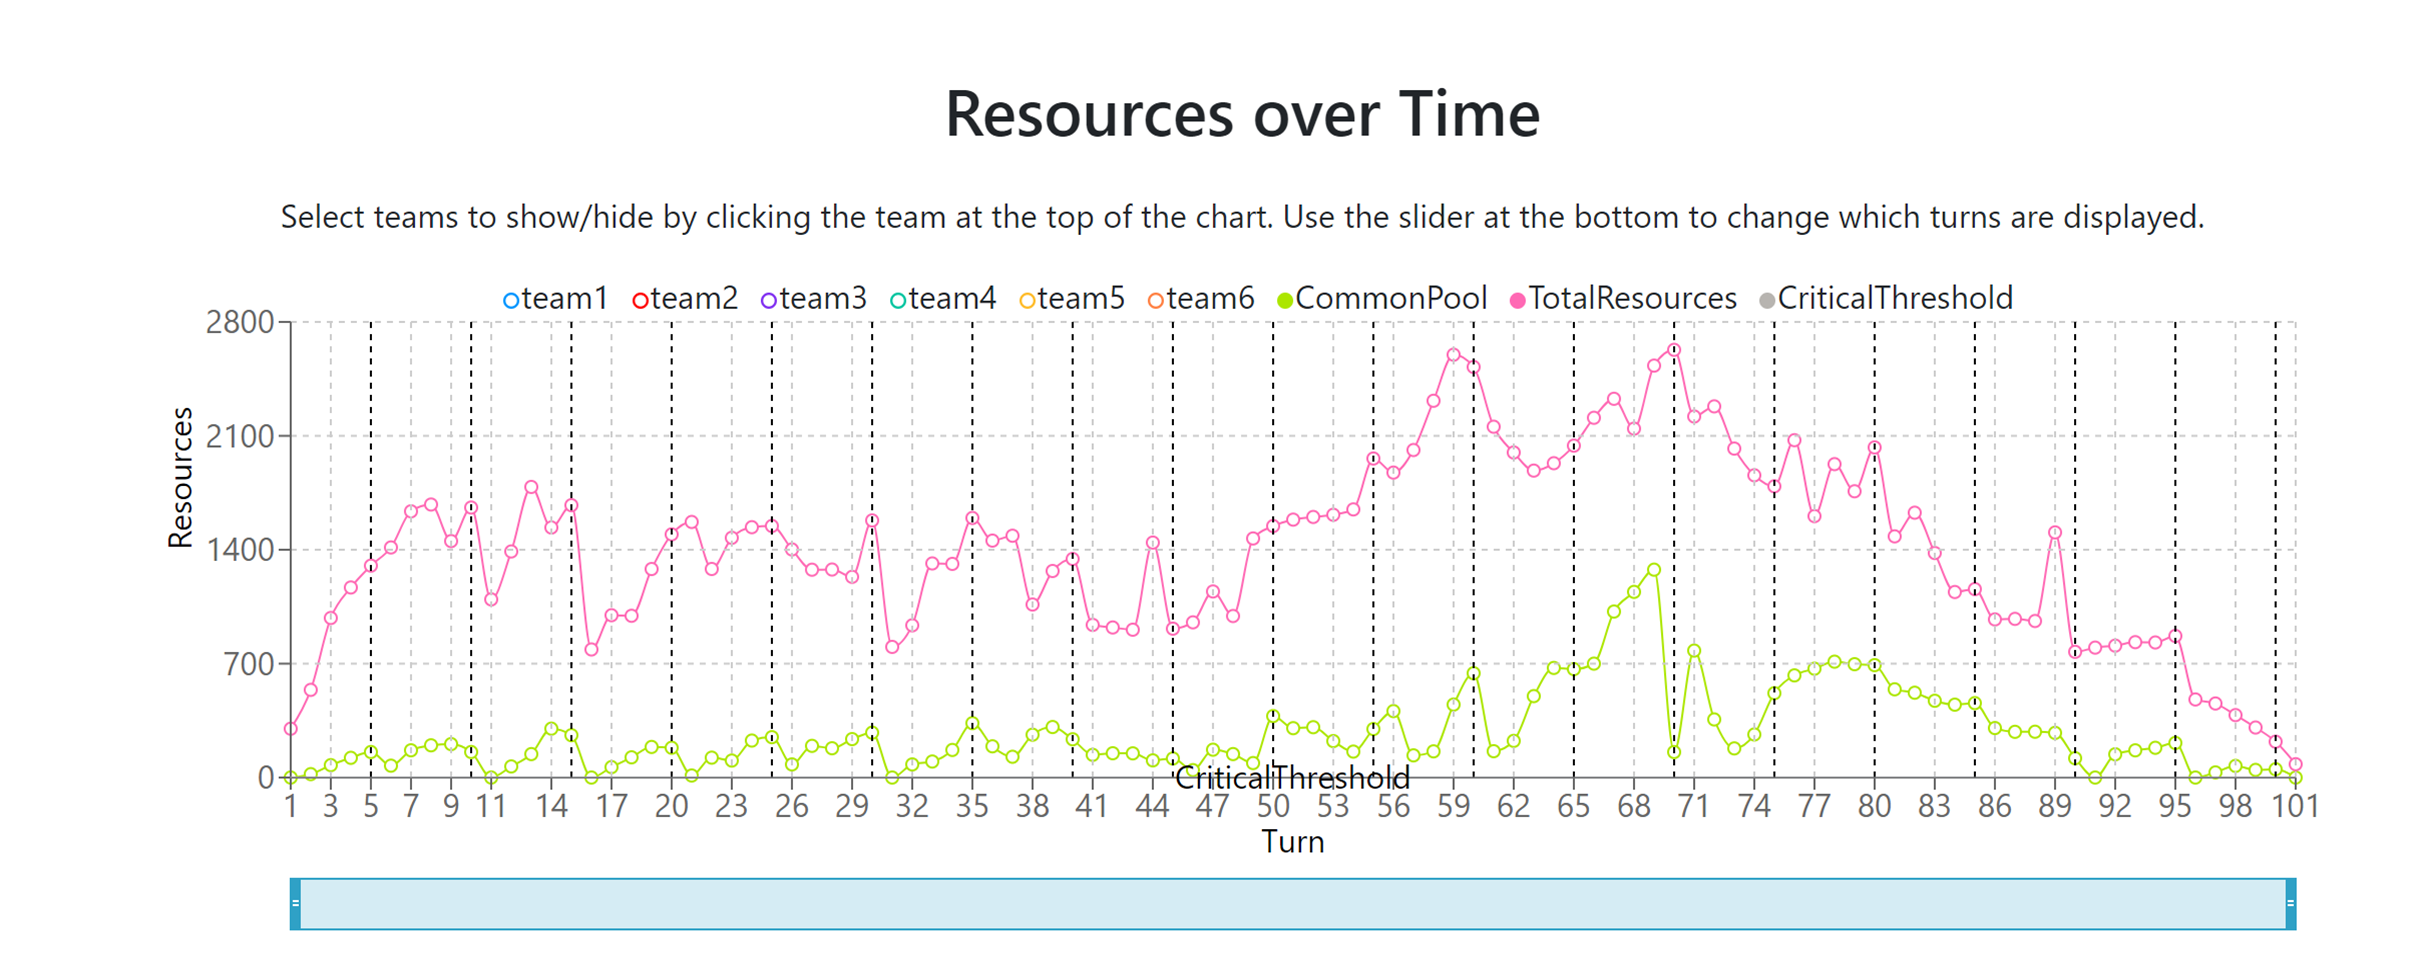
\includegraphics[width=\linewidth]{21_appendix_simulation/images/CPVisible.png}
    \caption{Common Pool Visible, with common pool threshold = 200}
    \label{fig:AppendixSim:cpvisible}
\end{figure}

\section{Disasters}
\subsection{Mag =50}
In this run most agents die on round 50 and then one agent survives and thrives, this simulation is used in \ref{tab:16_results_and_eval:Disasters:magnitude_period}
\begin{figure}[!htb]
    \centering
    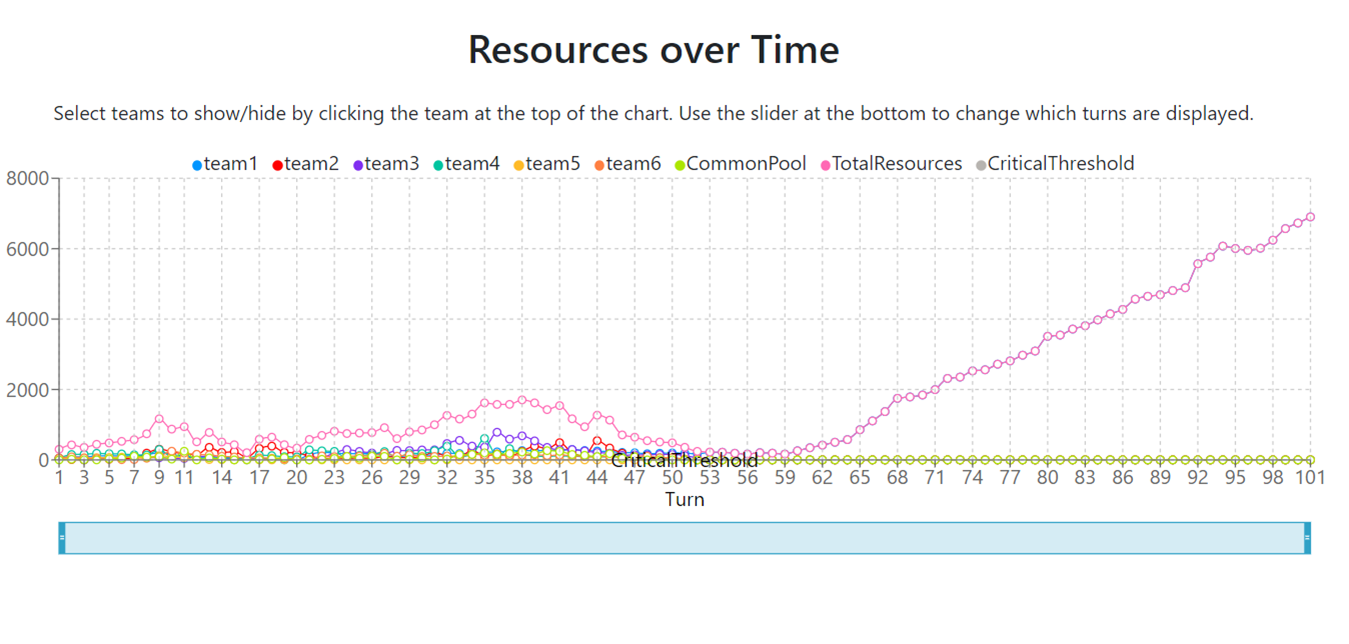
\includegraphics[width=\linewidth]{21_appendix_simulation/images/Mag=50.png}
    \caption{Disaster magnitude = 50, P = 1}
    \label{fig:AppendixSim:Disaster_mag50}
\end{figure}

\subsection{Mag =200}
In this run one agent keeps the islands alive for about 40 rounds then they are resurrected out of a sudden around turn 80. Great showcase of IITO and gifting. This data is used in \ref{tab:16_results_and_eval:Disasters:magnitude}
\ref{tab:16_results_and_eval:Disasters:magnitude}
\begin{figure}[!htb]
    \centering
    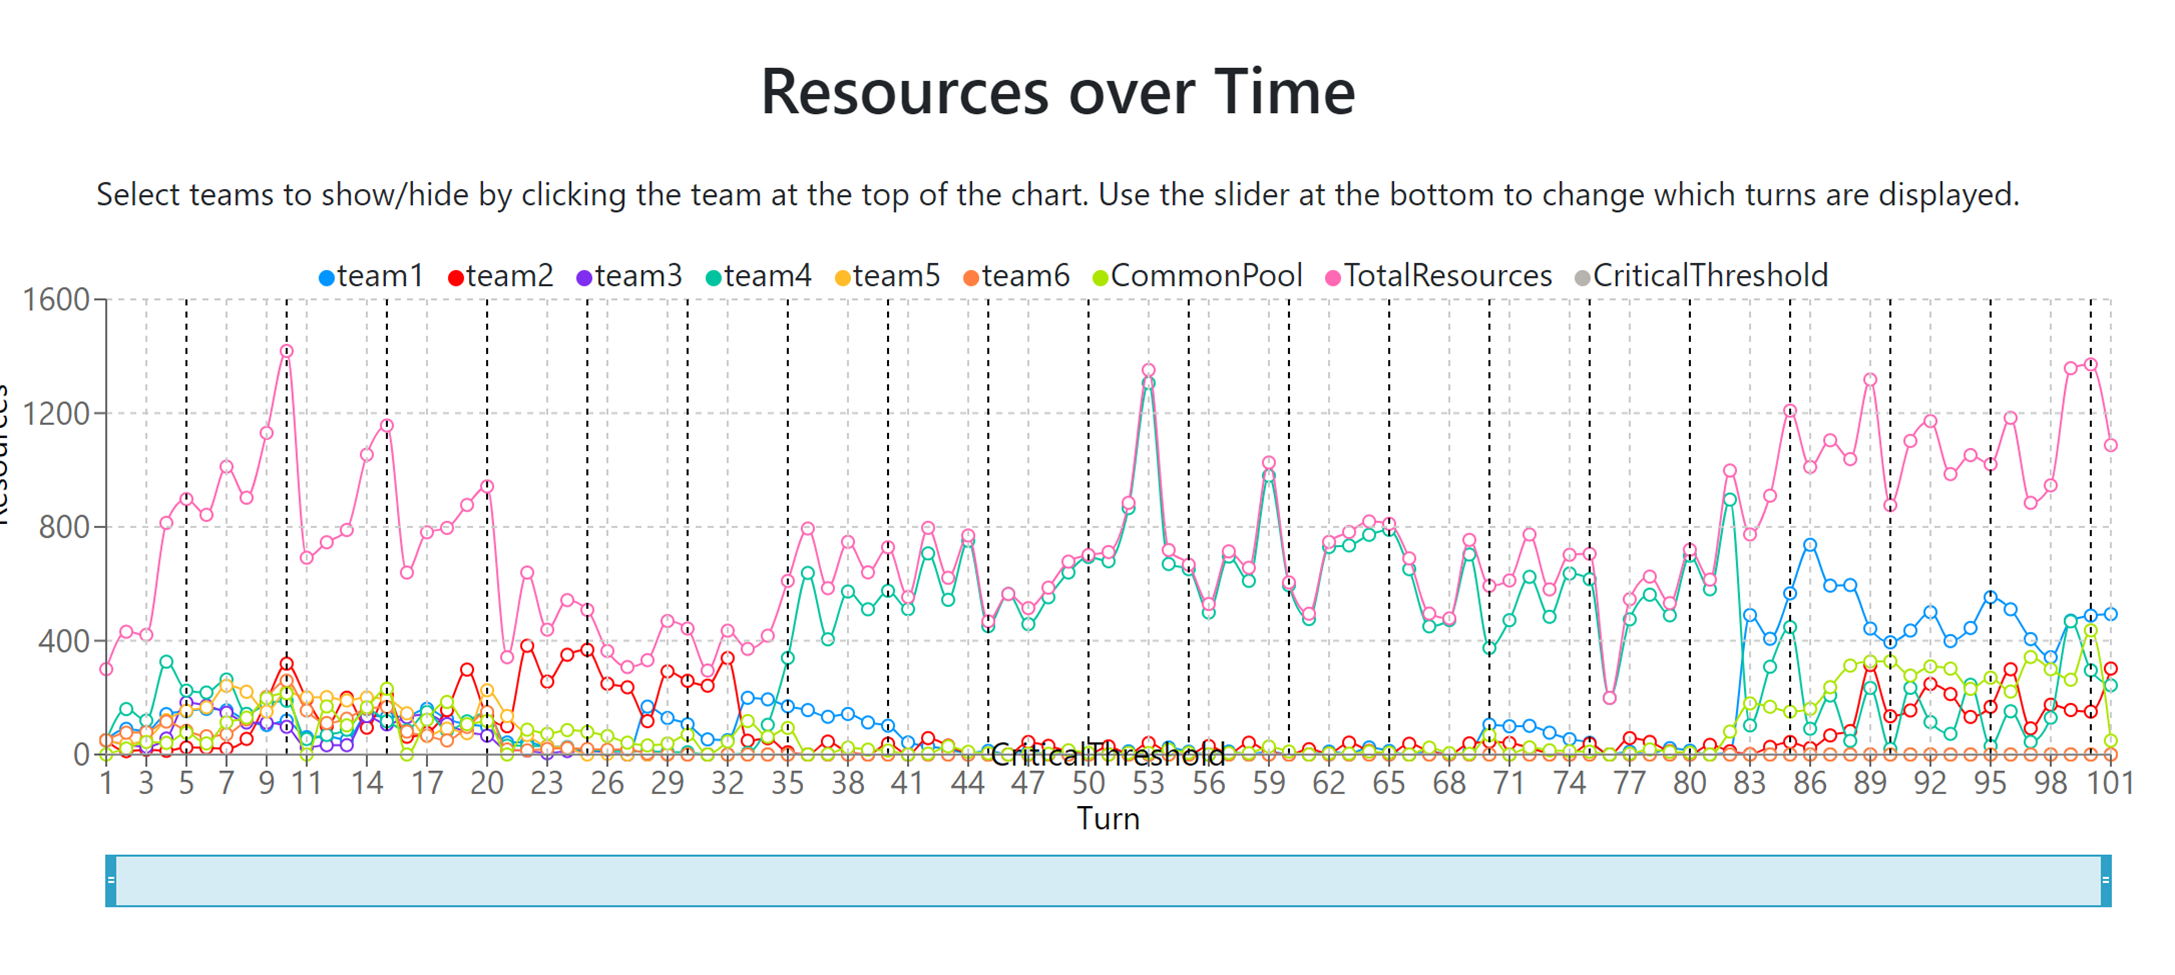
\includegraphics[width=\linewidth]{21_appendix_simulation/images/Mag=200.png}
    \caption{Disaster magnitude = 200}
    \label{fig:AppendixSim:Disaster_mag200}
\end{figure}


\subsection{Mag =500}
In this last one one agent is able to survive a big tragedy at the beginning, and then it survives for a while, but is not able to thrive in the same way that it did in \ref{fig:AppendixSim:Disaster_mag50}, this data is used in \ref{tab:16_results_and_eval:Disasters:magnitude}
\begin{figure}[!htb]
    \centering
    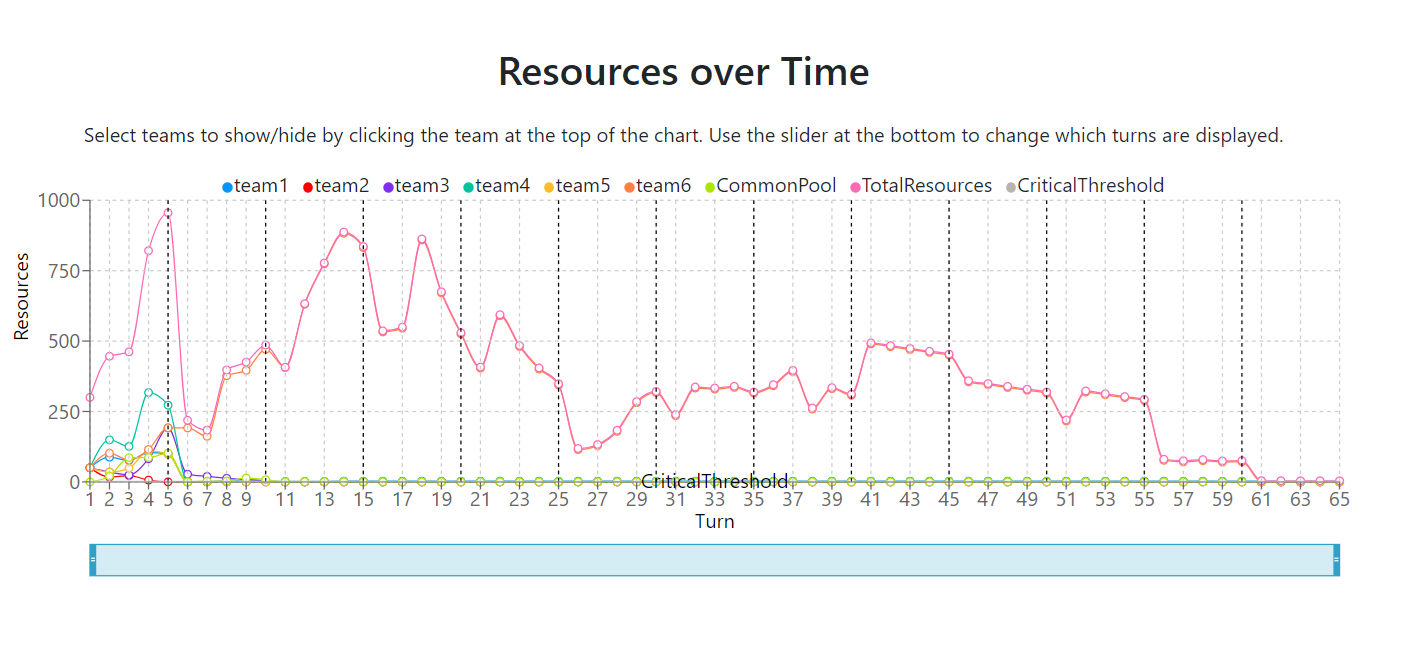
\includegraphics[width=\linewidth]{21_appendix_simulation/images/Mag=500.png}
    \caption{Disaster magnitude = 500}
    \label{fig:AppendixSim:Disaster_mag500}
\end{figure}